%==============================================================================
% CAPITOLUL 2 - Arhitectura sistemului (VARIANTA FARA COD)
% Toate listing-urile au fost mutate in Anexa A si Anexa B.
% In text se face referinta la Listing A.X / Listing B.X.
%==============================================================================


\chapter{Arhitectura sistemului}
\label{cap:arhitectura}

Acest capitol prezintă arhitectura platformei ETTIway, plecând de la o vedere de
ansamblu asupra componentelor și ajungând la detalierea fiecărui nivel al
sistemului. Sunt descrise separarea responsabilităților între frontend și
backend, structura datelor, mecanismul de autentificare și
autorizare. Totodată, sunt prezentate și fluxurile principale prin care componentele comunică între
ele. Deciziile de proiectare sunt motivate prin raportare la ideeile
formulate în capitolul anterior, cu accent pe securitate și
claritate a fluxului de utilizare. 
Fragmentele de cod care ilustrează aceste
mecanisme se găsesc în Anexa~A (cod Java pentru backend) și Anexa~B (cod
JavaScript pentru frontend).

\section{Vedere de ansamblu asupra arhitecturii}
\label{sec:ansamblu}

Platforma ETTIway este construită pe o arhitectură de tip client–server,
organizată pe trei niveluri logice distincte. Primul nivel este cel de
prezentare (frontend), realizat în HTML, CSS și JavaScript, care rulează în
browserul utilizatorului și se ocupă de afișarea hărții interactive, de
interacțiunea cu utilizatorul și de calculul traseelor. Al doilea nivel este
cel al serviciilor (backend), realizat cu Spring Boot, care expune servicii
web, gestionează autentificarea și autorizarea utilizatorilor și mediază
accesul la date. Al treilea nivel este cel al datelor, reprezentat de o bază
de date relațională PostgreSQL, în care sunt stocate atât conturile
utilizatorilor, cât și informația despre structura hărții.

Separarea pe aceste trei niveluri aduce mai multe avantaje. În primul rând,
permite dezvoltarea și testarea independentă a fiecărei componente, deoarece
interfața dintre niveluri este bine definită. În al doilea rând, izolează
logica de securitate la nivelul backend-ului, astfel încât regulile de acces
nu pot fi ocolite din interfața clientului. În al treilea rând, facilitează
extinderea sistemului: adăugarea de noi servicii sau de noi tipuri de date nu
necesită rescrierea componentelor existente, ci doar completarea celor noi.

Comunicarea dintre nivelul de prezentare și cel al serviciilor se realizează
prin cereri HTTP către un set de servicii de tip REST, datele fiind
transferate în format JSON. Această alegere asigură un cuplaj redus între
client și server: orice modificare internă a backend-ului rămâne transparentă
pentru frontend, atât timp cât contractul serviciilor este respectat.


\begin{figure}[H]
    \centering
    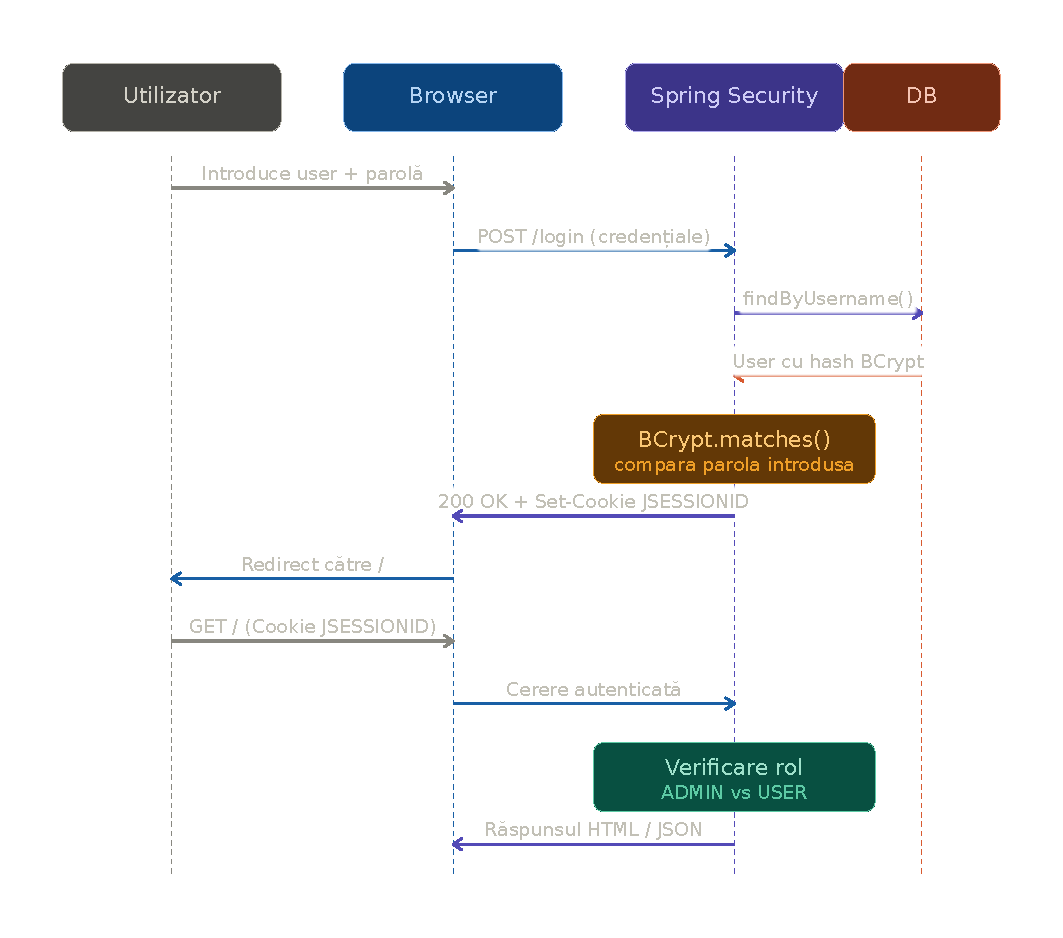
\includegraphics[width=0.80\textwidth]{figuri/flux_autentificare.pdf}
    \caption{Arhitectura sistemului ETTIway pe trei niveluri}
    \label{fig:flux-auth}
\end{figure}

\section{Nivelul de servicii (backend)}
\label{sec:backend}

Backend-ul aplicației este realizat cu ajutorul framework-ului Spring Boot \cite{Walls2022},
structurată pe pachete distincte în funcție de responsabilități. Pachetul de
configurare conține clasele de inițializare, de securitate și de pornire a
aplicației. Pachetul de entități conține clasele care modelează datele. Pachetul de repository conține interfețele de acces la baza de
date. Această organizare urmează convențiile de bază ale ecosistemului
Spring și face codul ușor de parcurs și de extins.

\subsection{Punctul de intrare al aplicației}
\label{subsec:punct-intrare}

Pornirea aplicației este gestionată de clasa principală, adnotată cu
\texttt{@SpringBootApplication}. Această adnotare activează mecanismele de
configurare automată ale Spring Boot, prin care componentele sunt descoperite
și inițializate fără configurare manuală explicită. Codul punctului de intrare
este minimal, întreaga logică de configurare fiind delegată claselor
specializate (vezi Listing~A.1 din Anexa~A). La pornire, pe lângă
inițializarea contextului Spring, aplicația execută și o componentă de
inițializare a datelor, care
asigură existența unui cont de administrator în baza de date.

\newpage
\subsection{Accesul la date prin JPA}
\label{subsec:jpa}

Accesul la baza de date se realizează prin intermediul JPA (Java Persistence
API) \cite{Walls2022}. În locul
scrierii manuale a interogărilor, accesul la date este definit prin interfețe
care extind \texttt{JpaRepository}, Spring generând automat implementările
necesare. Pentru utilizator, repository-ul definește în plus o
metodă de căutare după numele de utilizator, al cărei corp este generat
automat pe baza denumirii metodei (vezi Listing~A.2 din Anexa~A).

Avantajul acestei abordări este reducerea semnificativă a codului repetitiv:
operațiile uzuale de salvare, căutare și ștergere sunt moștenite din
\texttt{JpaRepository}, iar metodele specifice se declară prin simpla lor
semnătură. Tipul de retur \texttt{Optional} exprimă explicit faptul că un
utilizator căutat ar putea să nu existe, obligând codul apelant să trateze
acest caz și reducând astfel riscul de erori.

\subsection{Strategia de tratare a erorilor}
\label{subsec:erori}
 
Aplicația trebuie să gestioneze diverse situații de eroare, atât anticipate
(date invalide, resurse inexistente, autentificare eșuată), cât și
neanticipate (excepții la nivelul bazei de date, erori de rețea). În cadrul
ETTIway, tratarea erorilor a fost organizată pe trei niveluri, fiecare cu
rol distinct.
 
La nivelul backend-ului, controllerele REST returnează coduri HTTP
standardizate, conform convențiilor REST. Pentru operațiile reușite, codul
de răspuns este 200 (OK), pentru resursele inexistente 404 (Not Found),
pentru cererile invalide 400 (Bad Request), iar pentru tentativele de acces
neautorizat 401 (Unauthorized) sau 403 (Forbidden). Această standardizare
face ca frontend-ul să poată trata uniform diferitele tipuri de erori, fără
a se baza pe formate proprietare de mesaje.
 
La nivelul accesului la date, excepțiile aruncate de stratul JPA (de exemplu,
violări de constrângeri de unicitate, conexiuni întrerupte) sunt prinse în
blocurile try-catch ale serviciilor și transformate în răspunsuri HTTP
adecvate. De exemplu, o tentativă de a crea un cont cu un nume de utilizator
deja existent este detectată prin excepția de violare a constrângerii
\texttt{UNIQUE} pe coloana \texttt{username} și convertită într-un cod 400.
 
La nivelul frontend-ului, fiecare apel către API este însoțit de un bloc
\texttt{.catch} care interceptează erorile de rețea sau erorile returnate de
server. În cazul în care o operație eșuează, utilizatorului i se afișează o
fereastră modală cu un mesaj clar și acționabil, în loc de a-l lăsa în fața
unei interfețe care pare să nu răspundă. Aceste mesaje sunt formulate într-un
limbaj accesibil, evitând termenii tehnici care nu ar fi de folos
utilizatorului obișnuit.
 
Această abordare pe trei niveluri urmărește principiul \textit{fail fast}:
erorile sunt detectate și raportate cât mai aproape de sursa lor, fără a
permite propagarea unor stări inconsistente prin aplicație. În același timp,
prin folosirea codurilor HTTP standard, sistemul rămâne deschis pentru
integrarea ulterioară cu alți clienți (de exemplu, o aplicație mobilă nativă)
fără a impune un format propriu de comunicare.

\section{Nivelul de date}
\label{sec:date}

Datele sunt stocate într-o bază de date relațională PostgreSQL
\cite{PostgreSQL}, aleasă pentru suportul robust al tipurilor de date și pentru caracterul său open-source. Maparea dintre tabelele
bazei de date și obiectele din aplicație este realizată prin adnotări JPA pe
clasele de tip entitate. În cadrul ETTIway există două entități principale:
utilizatorii și datele hărții campusului, aceasta din urmă stocând atât
informația despre exterior, cât și planurile de etaj din interior.


\subsection{Alegerea bazei de date}
\label{subsec:alegere-db}
 
Pe parcursul analizei tehnologice am evaluat mai multe variante pentru
componenta de persistență a datelor, comparând atât baze de date relaționale,
cât și soluții de tip NoSQL. Această secțiune sintetizează compromisurile
considerate și justifică alegerea finală.
 
Alternativa cea mai evidentă a fost o bază de date relațională clasică, fie
PostgreSQL, fie MySQL. Ambele oferă maturitate, performanță și un ecosistem
solid de unelte și biblioteci. Comparativ, MySQL este mai răspândit în
aplicații web mai simple, iar PostgreSQL excelează în suportul pentru tipuri
de date avansate, în special pentru câmpurile JSON, pentru indexare flexibilă
și pentru extensibilitate. Având în vedere că structura datelor stocate de
ETTIway include atât valori scalare clasice (nume utilizator, parolă, rol),
cât și documente JSON complexe (graful campusului, planurile indoor),
PostgreSQL a fost mai bine adaptat pentru cerințele aplicației.
 
O a doua opțiune evaluată a fost o bază de date orientată pe documente, cum
sunt MongoDB sau CouchDB. Aceste sisteme sunt construite în jurul ideii de
stocare flexibilă a documentelor JSON, fără schemă fixă, ceea ce ar fi
corespuns natural modelului adoptat pentru graful și planurile indoor. În
schimb, ele introduc dependențe suplimentare, complexitatea unei tehnologii
separate pentru fiecare tip de date și necesitatea de a gestiona două sisteme
diferite în deployment (unul pentru utilizatori și autentificare, unul pentru
datele geospațiale). Pentru un proiect de această dimensiune, această
diversificare nu se justifică.
 
O a treia opțiune, considerată dar respinsă, a fost SQLite. SQLite este o
bază de date integrată direct în aplicație, fără server separat, ceea ce
simplifică dezvoltarea. Totuși, modelul său de concurență (un singur
scriitor activ la un moment dat) o face mai puțin potrivită pentru o
aplicație web care trebuie să gestioneze cereri simultane de la mai mulți
utilizatori. În plus, SQLite nu oferă mecanismele de gestionare a
utilizatorilor și a privilegiilor pe care PostgreSQL le pune la dispoziție
nativ.
 
Astfel, am ales PostgreSQL pentru combinația sa unică: stabilitatea unei baze
relaționale tradiționale, suportul pentru documente JSON la nivel de coloană
care a permis stocarea flexibilă a grafului, și disponibilitatea ca soluție
deschisă, gratuită și matură. Mai mult, această alegere lasă deschisă o
direcție viitoare de optimizare prin trecerea de la tipul de date \texttt{TEXT}
(folosit în versiunea actuală) la tipul nativ \texttt{JSONB}, care oferă
indexare în interiorul documentelor JSON și interogări mai eficiente, fără
să necesite o modificare arhitecturală a aplicației.


\subsection{Entitatea utilizator}
\label{subsec:user-entity}

Entitatea \texttt{User} modelează un cont din sistem și este mapată pe tabelul
\texttt{users}. Fiecare utilizator are un
nume de utilizator unic, o parolă stocată în formă criptată și un rol care
determină nivelul de acces. Constrângerile de unicitate și de obligativitate
sunt exprimate direct prin adnotări la nivel de coloană (vezi Listing~A.3 din
Anexa~A).

Constructorul fără argumente este necesar pentru ca JPA să poată instanția
obiectul atunci când citește o înregistrare din baza de date, iar metodele de
tip getter și setter permit citirea și scrierea câmpurilor. Parola nu este
niciodată stocată în clar, ci doar în forma sa criptată, aspect detaliat în
secțiunea despre securitate.
\newpage
\subsection{Entitatea pentru datele hărții}
\label{subsec:mapdata-entity}

A doua entitate, \texttt{MapData}, este responsabilă de persistarea structurii
hărții campusului. Pentru a permite o reprezentare flexibilă a grafului de
noduri și muchii pe care se bazează rutarea, structura este serializată în
format JSON și stocată într-o coloană de tip text. Aceeași entitate cuprinde
și planurile de etaj din interior, păstrate într-o a doua coloană JSON
distinctă. Această abordare unificată evită multiplicarea tabelelor pentru
date conceptual înrudite și permite modificarea structurii grafului sau a
planurilor indoor fără a fi necesare migrări ale schemei relaționale (vezi
Listing~A.4 din Anexa~A).

Cele două câmpuri JSON sunt însoțite de un câmp pentru momentul ultimei
actualizări, util pentru urmărirea modificărilor aduse hărții. Stocarea
flexibilă ca documente JSON constituie o decizie de proiectare orientată spre
extensibilitate: noduri, muchii sau planuri de etaj pot fi adăugate ori
modificate fără a impune o structură fixă la nivelul tabelelor.

\subsection{Reprezentarea planurilor de etaj}
\label{subsec:indoor-storage}

Planurile de etaj sunt organizate ierarhic în câmpul \texttt{indoorJson} al
entității \texttt{MapData}, sub forma unui obiect care asociază fiecărei
clădiri lista etajelor sale. Fiecare etaj conține un document GeoJSON cu
toate elementele desenate de administrator: camerele (poligoane închise, cu
nume), nodurile (puncte de pe coridoare, având tipuri distincte pentru
intrare în cameră, intersecție sau scară) și muchiile (linii care leagă două
noduri și reprezintă un segment de coridor). Această organizare păstrează
consistența cu modelul folosit pentru harta exterioară și permite reutilizarea
aceleiași logici de prelucrare GeoJSON la nivelul clientului.


\subsection{Strategia de modelare a datelor}
\label{subsec:strategie-date}
 
Decizia de a stoca atât graful campusului, cât și planurile indoor sub formă
de documente JSON serializate ca text, în loc de a folosi o schemă relațională
clasică cu mai multe tabele, nu a fost aleasă întâmplător.
Modelul ales este similar conceptului de \textit{document store}, utilizat de
baze de date precum MongoDB sau CouchDB, dar implementat peste o bază relațională
clasică, beneficiind astfel de fiabilitatea PostgreSQL fără a renunța la
flexibilitatea schemei.
 
Avantajul principal al acestei abordări este că structura datelor poate evolua
fără modificări de schemă în baza de date. Adăugarea unui nou tip de element
(de exemplu, un punct de interes cu proprietăți noi) sau a unui atribut
suplimentar pentru o cameră (de exemplu, capacitate, accesibilitate, ore de
funcționare) nu necesită alterarea tabelului prin instrucțiuni
\texttt{ALTER TABLE}. Frontend-ul și logica de
prelucrare a JSON-ului sunt singurele componente care trebuie ajustate.
 
Alternativa relațională ar fi presupus tabele separate pentru clădiri, etaje,
camere, noduri și muchii, legate prin chei străine. O astfel de schemă oferă
posibilitatea unor interogări complexe la nivelul bazei de date (de exemplu,
filtre după proprietăți specifice ale camerelor, agregări per clădire). Acest lucru
introduce o rigiditate care nu se justifică în contextul actual al aplicației.
Pentru ETTIway, interogările sunt simple: încărcarea în memorie a întregului
document și prelucrarea sa la nivelul aplicației. Volumul de date asociat unui
campus universitar (câteva sute de clădiri, câteva mii de noduri) face ca
această încărcare integrală să fie eficientă, sub un megabyte de JSON pentru un
campus de talie medie.
 
Un al doilea avantaj al modelului este simplitatea persistenței: tot graful
exterior sau toate planurile indoor ale unei clădiri sunt salvate printr-o
singură operație de scriere în baza de date. Această automatizare evită
problemele de consistență care apar într-un model relațional, în care
salvarea unui graf complet ar însemna multiple operații de inserare în mai
multe tabele, cu necesitatea folosirii tranzacțiilor pentru a garanta
integritatea. Aceasta automatizare naturală a stocării JSON face logica de salvare
mai simplă atât în backend, cât și în frontend.
 


\section{Securitate: autentificare și autorizare}
\label{sec:securitate}

Un aspect central al arhitecturii ETTIway îl constituie mecanismul de
securitate, care diferențiază între utilizatorii obișnuiți și administratori.
Această diferențiere este esențială, deoarece administratorii pot modifica
structura hărții, în timp ce utilizatorii obișnuiți au acces doar în mod de
vizualizare. Securitatea este implementată folosind Spring Security
\cite{SpringSecurity}, integrat nativ în ecosistemul Spring Boot.

\subsection{Criptarea parolelor}
\label{subsec:bcrypt}
 
Parolele utilizatorilor nu sunt stocate în clar în baza de date, ci sunt
criptate folosind algoritmul BCrypt \cite{BCrypt}, prin intermediul unei
componente dedicate de codare a parolelor. BCrypt este un algoritm de tip
funcție de derivare a cheii, conceput special pentru stocarea parolelor: el
este lent în mod intenționat și încorporează un factor aleatoriu, ceea ce
îngreunează semnificativ atacurile prin forță brută.
 
\begin{figure}[H]
    \centering
    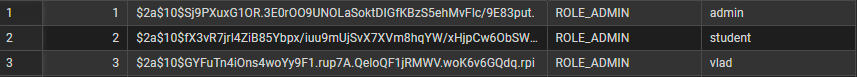
\includegraphics[width=0.8\textwidth]{figuri/Tabel Utilizatori.png}
    \caption{Structura tabelului de utilizatori în baza de date, evidențiind câmpurile pentru numele de utilizator, parola criptată și rolul asociat.}
    \label{fig:2.a}
\end{figure}

Alegerea BCrypt în detrimentul altor funcții de hash a fost una conștientă.
Funcțiile generale de hash criptografic, precum MD5 sau SHA-256, sunt
proiectate pentru a fi rapide, ceea ce le face potrivite pentru verificarea
integrității fișierelor sau pentru semnături digitale, dar dezavantajoase
pentru stocarea parolelor. Viteza lor permite unui atacator cu hardware
modern să calculeze miliarde de hash-uri pe secundă, ceea ce face fezabile
atacurile prin dicționar pe parole obișnuite. BCrypt, în schimb, este
proiectat să fie lent prin construcție și are doi parametri suplimentari
care îi conferă rezistența: \textit{salt}-ul și \textit{cost factor}-ul.
 
\textit{Salt}-ul este o secvență aleatoare care este atașată parolei înainte
de calculul hash-ului. Acest mecanism garantează că două parole identice
produc hash-uri diferite și, mai important, blochează atacurile cu
\textit{rainbow tables}, care sunt tabele precalculate de hash-uri pentru
parolele uzuale. Fiecare hash BCrypt include automat un salt unic, generat
aleator la criptare, ceea ce înseamnă că dezvoltatorul nu trebuie să se
preocupe explicit de gestionarea sa. Salt-ul este stocat ca parte a hash-ului
final, iar la verificare este extras automat pentru a recompune comparația.
 
\textit{Cost factor}-ul controlează numărul de iterații pe care le execută
algoritmul. La fiecare incrementare a valorii cu 1, calculul durează de două
ori mai mult, conform unei progresii exponențiale. Configurația implicită
folosită în Spring Security 6 este 10, ceea ce înseamnă $2^{10} = 1024$ de
iterații pentru fiecare verificare. Pe hardware modern, această configurație
oferă un timp de verificare de aproximativ o sutime de secundă, suficient de
rapid pentru un login normal, dar suficient de lent încât atacurile prin forță
brută să fie costisitoare. Pe măsură ce hardware-ul devine mai rapid, valoarea
acestui parametru poate fi crescută fără modificări structurale ale aplicației
sau ale bazei de date.
 
Componenta de criptare este definită ca un bean Spring (vezi Listing~A.5 din
Anexa~A), ceea ce permite injectarea sa automată în orice altă componentă
care are nevoie de criptarea sau verificarea parolelor. La crearea unui cont,
parola este trecută prin această componentă înainte de a fi salvată, iar la
autentificare, parola introdusă este comparată cu cea criptată din baza de
date prin metoda \texttt{matches}, care extrage automat salt-ul și cost
factor-ul din hash-ul stocat și recompune verificarea.
 
În cazul în care, la o dată viitoare, BCrypt ar fi considerat depășit, Spring
Security oferă mecanisme de migrare progresivă a hash-urilor către un alt
algoritm prin componenta 
\texttt{\seqsplit{DelegatingPasswordEncoder}}. Fără a impune
resetarea tuturor parolelor existente. Această flexibilitate, oferită prin
prefixarea hash-urilor cu un identificator de algoritm, asigură că soluția
adoptată astăzi nu blochează evoluții ulterioare ale platformei.
 

\subsection{Configurarea regulilor de acces}
\label{subsec:reguli-acces}

Regulile care stabilesc ce resurse sunt accesibile public, ce resurse necesită
autentificare și ce resurse sunt rezervate administratorilor sunt definite
într-un lanț de filtre de securitate (vezi Listing~A.6 din Anexa~A).
Resursele statice și paginile de autentificare sunt publice, rutele
administrative sunt rezervate utilizatorilor cu rol de administrator, iar
restul paginilor necesită cel puțin autentificare.

Autentificarea propriu-zisă se realizează printr-un formular de login,
configurat să folosească o pagină proprie și să redirecteze utilizatorul,
după succes, către o rută care verifică rolul acestuia și îl direcționează
corespunzător. Deconectarea invalidează sesiunea și readuce utilizatorul la
pagina de autentificare.

\subsection{Încărcarea utilizatorilor și inițializarea contului de administrator}
\label{subsec:init-admin}

Pentru ca Spring Security să poată verifica identitatea unui utilizator, este
necesară o componentă care să încarce datele acestuia din baza de date pe
baza numelui de utilizator. Această componentă implementează interfața
\texttt{UserDetailsService} și transformă entitatea proprie \texttt{User}
într-un obiect pe care mecanismul de securitate îl poate folosi, inclusiv
rolul asociat (vezi Listing~A.7 din Anexa~A).

Pentru a asigura existența unui cont de administrator încă de la prima
pornire a aplicației, este folosită o componentă de inițializare care se
execută automat la lansare. Aceasta verifică dacă există deja un cont de
administrator și, în caz contrar, îl creează, criptând în prealabil parola
(vezi Listing~A.8 din Anexa~A). Astfel, sistemul devine utilizabil imediat
după instalare, fără a necesita o configurare manuală a bazei de date. Acest
mecanism ilustrează un principiu de proiectare orientat spre ușurința punerii
în funcțiune: starea minimă necesară funcționării sistemului este creată
automat, reducând efortul de configurare și posibilitatea unor erori manuale.

\section{Nivelul de prezentare (frontend)}
\label{sec:frontend}

Nivelul de prezentare este realizat în JavaScript, folosind biblioteca Leaflet
\cite{Leaflet} pentru afișarea hărții interactive. Pe lângă afișarea
propriu-zisă, frontend-ul încorporează și o parte importantă din logica
aplicației, în special construirea grafului de navigare și calculul
traseelor. Această secțiune descrie elementele principale ale interfeței și
mecanismele de prelucrare implementate pe partea de client.
\newpage
\subsection{Inițializarea hărții și delimitarea zonei}
\label{subsec:init-harta}

Harta este centrată pe coordonatele campusului și limitată la o zonă
geografică bine definită, pentru a împiedica utilizatorul să navigheze în
afara regiunii de interes. Coordonatele de centrare și limitele zonei sunt
definite ca valori de configurare (vezi Listing~B.1 din Anexa~B).

Pe lângă afișarea hărții, interfața include un panou lateral care găzduiește
funcțiile de căutare, lista clădirilor disponibile și detaliile clădirii. Detaliile despre o sală cum ar fi: clădirea, etajul
și tipul sunt generate dinamic, cu prelucrarea atentă a textului pentru a
preveni problemele de afișare și eventualele riscuri de securitate, prin
transformarea caracterelor speciale înainte de inserarea în pagină.

\subsection{Construirea grafului de navigare}
\label{subsec:graf}

Pentru a putea efectua calculul traseelor între puncte, infrastructura campusului
este transformată într-un graf, în care nodurile reprezintă intersecții sau
puncte de pe trasee, iar muchiile reprezintă segmentele care le leagă.
Graful este construit pornind de la datele geografice exprimate în format
GeoJSON \cite{GeoJSON}, în care elementele de tip linie descriu aleile și
drumurile.

Fiecare nod este identificat printr-o cheie obținută din coordonatele sale,
rotunjite la o precizie fixă, pentru a asigura că puncte foarte apropiate
sunt tratate ca un singur nod. Pentru fiecare segment al unei linii se
adaugă o muchie între nodurile adiacente, ponderea muchiei fiind distanța
geografică reală dintre cele două puncte. Graful rezultat este
nedirecționat, deoarece o alee poate fi parcursă în ambele sensuri.
Implementarea construirii grafului este prezentată în Listing~B.2 din
Anexa~B. Observația importantă privind formatul GeoJSON este că acesta
exprimă coordonatele în ordinea longitudine–latitudine, în timp ce Leaflet le
așteaptă în ordinea latitudine–longitudine. Conversia corectă între cele două
este necesară pentru ca punctele să fie plasate corect pe hartă.

\subsection{Calculul traseului prin algoritmul Dijkstra}
\label{subsec:dijkstra}

Determinarea celui mai scurt traseu între două puncte se realizează prin
algoritmul Dijkstra, implementat direct pe partea de client (vezi
Listing~B.3 din Anexa~B). Plecând de la nodul de start, algoritmul menține
pentru fiecare nod distanța minimă cunoscută și nodul precedent pe traseul
optim. Apoi alege la fiecare pas nodul nevizitat cu distanța cea mai mică și
actualizează distanțele vecinilor săi. Atunci când nodul de destinație este
atins, traseul este reconstruit parcurgând în sens invers lanțul nodurilor
precedente.

Deoarece punctele alese de utilizator nu coincid, în general, exact cu
nodurile grafului, este necesară o etapă de asociere a fiecărui punct cu cel
mai apropiat nod existent (vezi Listing~B.4 din Anexa~B). Aceasta se
realizează printr-o căutare a nodului aflat la distanța minimă față de
punctul țintă, asigurând că rutarea pornește și se încheie în puncte aflate
efectiv pe rețeaua de trasee. Dacă între cele două puncte nu există niciun
traseu - de exemplu, atunci când o porțiune a rețelei este izolată -
algoritmul returnează o valoare care semnalează absența unei rute, iar
interfața poate informa utilizatorul în consecință.

\newpage

\section{Fluxul de comunicare între componente}
\label{sec:flux}

Reunind cele trei niveluri, fluxul tipic de utilizare al aplicației poate fi
descris astfel. La accesarea aplicației, utilizatorul este direcționat către
pagina de autentificare.În cele ce urmează se validează credențialele de către backend,
rolul său determină modul de funcționare: vizualizare pentru utilizatorii
obișnuiți, respectiv editare pentru administratori. Frontend-ul solicită apoi
structura hărții de la backend, care o extrage din baza de date și o
transmite în format JSON. Pe baza acestor date, clientul construiește graful
de navigare și afișează harta interactivă.

\begin{figure}[H]
    \centering
    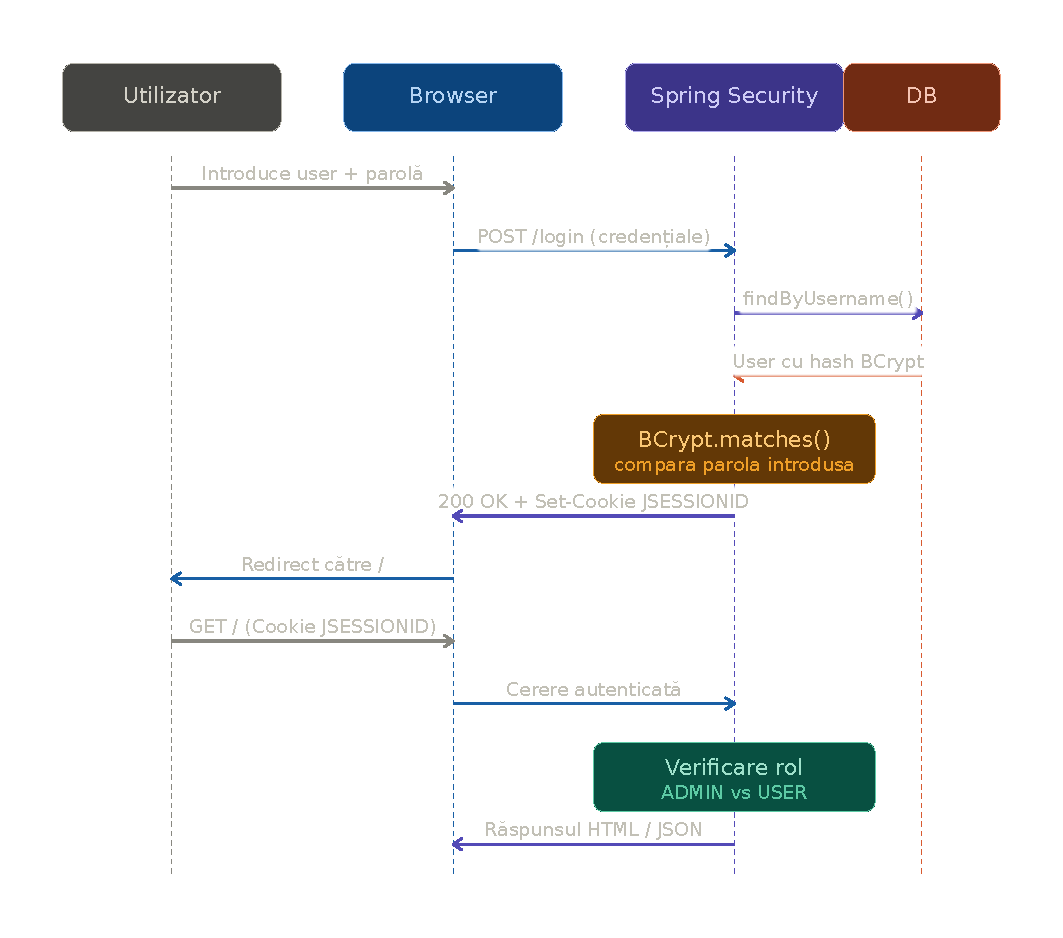
\includegraphics[width=0.80\textwidth]{figuri/flux_autentificare.pdf}
    \caption{Fluxul detaliat de autentificare al unei cereri HTTP}
    \label{fig:flux-auth}
\end{figure}

Atunci când utilizatorul selectează un punct de plecare și unul de
destinație, calculul traseului se realizează integral pe partea de client,
prin construirea grafului, asocierea punctelor cu cele mai apropiate noduri
și aplicarea algoritmului Dijkstra. Această alegere reduce sarcina
serverului și asigură un timp de răspuns redus.Traseul este calculat și
afișat fără a necesita o nouă cerere către backend. Modificările aduse
structurii hărții de către un administrator sunt, în schimb, transmise către
backend și stocate în baza de date, devenind astfel disponibile tuturor
utilizatorilor la accesările ulterioare.


\newpage
\section{Concluziile capitolului}
\label{sec:concluzii-cap2}

În acest capitol a fost prezentată arhitectura platformei ETTIway, organizată
pe trei niveluri: prezentare, servicii și date. A fost descris backend-ul
realizat cu Spring Boot, cu accesul la date prin JPA și cu stocarea de date în
PostgreSQL. Precum și cele două entități principale ale sistemului - pentru
utilizatori și pentru datele hărții campusului. Aceasta din urmă cuprinzând
atât informația despre exterior, cât și planurile de etaj din interior. 
S-a detaliat mecanismul de securitate, bazat pe Spring Security, cu
criptarea parolelor prin BCrypt. Am prezentat si diferențierea rolurilor și inițializarea
automată a contului de administrator. La nivelul de prezentare au fost
prezentate inițializarea hărții, construirea grafului de navigare din date
GeoJSON și implementarea algoritmului Dijkstra pentru calculul traseelor.

Deciziile de proiectare descrise - separarea pe niveluri, stocarea flexibilă
a grafului, calculul traseelor pe partea de client și inițializarea automată
a sistemului - au fost orientate spre extensibilitate, securitate și ușurința
punerii în funcțiune. Capitolul următor abordează
modul concret de utilizare a aplicației și rezultatele obținute, ilustrând
funcționarea sistemului în scenariile reale de navigare din campus,
incluzând și rutarea în interiorul clădirilor.
